\chptr{Alberi}

\section{Alberi e proprietà}

\begin{tcolorbox}[colback=yellow!30, colframe=yellow!30!black, title = {Alberi e Foreste}]
\begin{itemize}
    \item \textbf{Foresta}: un grafo senza cicli.
    \item \textbf{Albero}: un grafo \textit{connesso} e senza cicli.
\end{itemize}
\end{tcolorbox}

\begin{osservaz}
Un grafo è una foresta se e solo se ogni sua componente connessa è un albero.

Sia infatti $G$ un grafo con proprietà di foresta; allora $G$ è un grafo senza
cicli; se $G$ è connesso, allora esso è anche un albero; altrimenti, $G$ è
costituito da più di una componente connessa; essendo $G$ senza cicli per
ipotesi, ogni componente di $G$ deve essere un albero. Si supponga ora che
$G$ sia un grafo connesso con proprietà di albero; $G$ allora non ha cicli
ed è una foresta; sia invece $G$ sconnesso tale per cui ogni componente
sia un albero; allora ogni componente di $G$ (e $G$ stesso) non ha cicli
e quindi è una foresta.
\end{osservaz}

\subsection*{Teorema sugli alberi}
Sia $T=(V,E)$ un grafo non connesso finito. Le seguenti affermazioni
sono equivalenti:
\begin{enumerate}
\item $T$ è un albero.
\item $\forall v,v'\in V, \exists!$ cammino in $T$ che congiunge $v,v'$.
\item \textbf{Minimalità della connessione:}

$T$ è connesso e $\forall e\in E, T-e:=(V,E\setminus \{e\})$ è sconnesso.


\item \textbf{Massimalità rispetto all'assenza di cicli:}

$T$ non ha cicli e $\forall e \in \binom{V}{2}\setminus E, T+e:=(V,E\cup\{e\})$ possiede cicli.
\end{enumerate}

\subsection*{Lemma delle foglie}
Sia $T$ un albero finito avente almeno due vertici. Allora $T$ possiede almeno
due foglie.
$\\\\$
\textit{\textbf{Dimostrazione:}} Sia $\mathcal{P}$ l'insieme di  tutti i cammini
possibili in $T$. Poiché $T$ è finito, $\mathcal{P}$ è finito. Dunque esiste un
cammino $P=(v_0,...,v_k) \in \mathcal{P}$ che abbia lunghezza massima $k$:
\[ k=l(P)\geq l(P') \quad \forall P'\in\mathcal{P} \]
Dimostriamo che $v_0,v_k$ sono due foglie di $T$. Supponiamo che $v_0$ non sia
una foglia. Quindi $\deg_T(v_0)\geq 2$. Sia allora $v'$ vertice del secondo
lato $\{v_0,v'\}$. $v'\not\in\{v_1,...,v_k\}$, perché altrimenti si creerebbero
cicli. Ma allora si otterrebbe una passeggiata $P'=(v',v_0,...,v_k)$ di lunghezza
maggiore di $P$. Quindi necessariamente $\deg_T(v_0)=1$.
\cvd


\begin{osservaz}
Il \textit{Lemma delle foglie} è falso se non si assume che l'albero sia
finito. Esistono alberi infiniti che possiedono una o nessuna foglia
(si prenda come esempio un cammino infinito).
\end{osservaz}


\subsection*{Lemma della rimozione delle foglie (ex 20.8)}
Se $G$ è un grafo connesso e $v$ è una sua foglia, allora $G - v$ è connesso.

\subsection*{Corollario della rimozione delle foglie (ex 20.9)}
Sia $T$ un albero e sia $v$ una sua foglia. Allora $T - v$ è ancora un albero.


\section{\underline{Alberi e formula di Eulero}}

\begin{tcolorbox}[
        enhanced,
        breakable,
        title={Teorema di caratterizzazione degli alberi finiti con formula di Eulero}
    ]
    Sia $T=(V,E)$ un grafo finito. Le seguenti affermazioni sono equivalenti:
    \begin{enumerate}
        \item $T$ è un albero;
        \item $\forall v,v'\in V,\exists! \text{ cammino in} T \text{ che congiunge} v,v'$;
        \item Minimalità della connessione;
        \item Massimalità rispetto all'assenza di cicli;
        \item \textbf{$T$ è connesso e vale la seguente formula di Eulero:}
    \end{enumerate}
    \[ |V|-1=|E| \]
    \textit{\textbf{Dimostrazione:}} Mostriamo che (1) $\Rightarrow$ (5). Procediamo
    per induzione su $|V(T)|$.
    \\\\
    $|V(T)|=1$ (\textbf{base induzione}): $T$ consiste in un vertice isolato, dunque $|V(T)|=1$ e $|E(T)|=0
    \Longrightarrow |V(T)|-1 = 1-1 = 0 = |E(T)|$.
    \\\\
    $|V(T)|\geq 2, |V(T)|-1\Longrightarrow|V(T)|$ (\textbf{passo induttivo}) Sia $T$ un albero con
    almeno 2 vertici. Assumiamo che la formula di Eulero valga su tutti gli alberi che
    possiedono un vertice in meno di $T$ (ipotesi induttiva). Grazie al lemma 20.6, $T$
    possiede almeno due foglie $v,w$. Grazie al \textit{Corollario della rimozione delle foglie},
    $T-v$ è un albero. Segue che $|V(T-v)|=|V(T)|-1$, dunque per ipotesi induttiva vale la formula di
    Eulero per $T-v$:
    \begin{align*}
        |V(T-v)|-1=|E(T-v)| \Longrightarrow 1&+|V(T-v)| - 1 = 1+|E(T-v)|\\
        &\Downarrow\\
        |V(T)|-1&=|E(T)|
    \end{align*}

    Il passo induttivo è verificato, dunque grazie al principio di induzione di prima forma
    l'implicazione (1)$\Rightarrow$(5) è sempre vera.
    \\\\
    Mostriamo ora che (5) $\Rightarrow$ (1). Procediamo per induzione su $|V(T)|$.
    \\\\
    $|V(T)|=1$ (base induzione): $T$ possiede un solo vertice: è un albero e vale (1).
    \\\\
    $|V(T)|\geq 2, |V(T)|-1\Longrightarrow|V(T)|$. Sia $T$ un grafo finito
    connesso con almeno due vertici e che soddisfa la formula di Eulero. Assumiamo che l'implicazione
    (5)$\Rightarrow$(1) sia vera per tutti i grafi finiti connessi con esattamente
    $|V(T)|-1$ vertici e per i quali vale la formula di Eulero (ipotesi induttiva).
    Mostriamo che $T$ ammette almeno una foglia.
    Supponiamo che $T$ non abbia foglie; segue che:
    \begin{align*}
        &\forall w\in V(T)\\
        &\deg_T(w)\not = 0 \text{ per ipotesi sulla connessione e sul numero minimo di vertici}\\
        &\deg_T(w)\not = 1 \text{ per supposizione sull'assenza di foglie}\\
        &\Longrightarrow \deg_T(w)\geq 2
    \end{align*}
    Vale, per ipotesi (vale Eulero per $T$)$^*$ e per la relazione fondamentale dei grafi finiti$^{**}$:
    \[ 2(|V(T)|-1)\stackrel{\text{*}}{=}2|E(T)|\stackrel{\text{**}}{=}\sum_{w\in V(T)}\deg_T(w)\geq \sum_{w\in V(T)}2=2|V(T)| \]
    Il che è assurdo, a causa del fatto che si è assunta l'assenza di foglie.
    Quindi $\exists v$ foglia di $T$. Allora per il \textit{Lemma della rimozione delle foglie}
    $T-v$ è connesso.
    Siccome $T$ soddisfa la formula di Eulero,
    \[ (|V(T)|-1) -1 = |E(T)|-1 \Rightarrow |V(T-v)|-1=|E(T-v)|\]
    quindi $T-v$ soddisfa la formula di Eulero
    e ad esso si può applicare l'ipotesi induttiva: $T-v$ è un albero. $T$ non
    può avere un ciclo, perché tale ciclo dovrebbe attraversare vertici di grado
    maggiore o uguale di 2, dunque non può attraversare la foglia. Ma per ipotesi
    $T-v$ è un albero, dunque tale ciclo non può esistere. Allora $T$ è un albero.
    Il passo induttivo è verificato, quindi l'implicazione inversa è sempre vera
    grazie al principio di induzione di prima forma.
    \cvd
\end{tcolorbox}



\section{\underline{Alberi di copertura}}
\begin{tcolorbox}[colback=yellow!30, colframe=yellow!30!black, title=Albero di copertura]
Sia $G$ un grafo. Un sottografo $T$ di $G$ è un albero di copertura (spannig tree) se:
\begin{itemize}
\item $T$ è un albero.
\item $V(T)=V(G)$
\end{itemize}
\end{tcolorbox}

La Figura \ref{spanning} mostra un grafo $G$ ed evidenzia un suo possibile
spanning tree.

\begin{figure}[H]
\centering
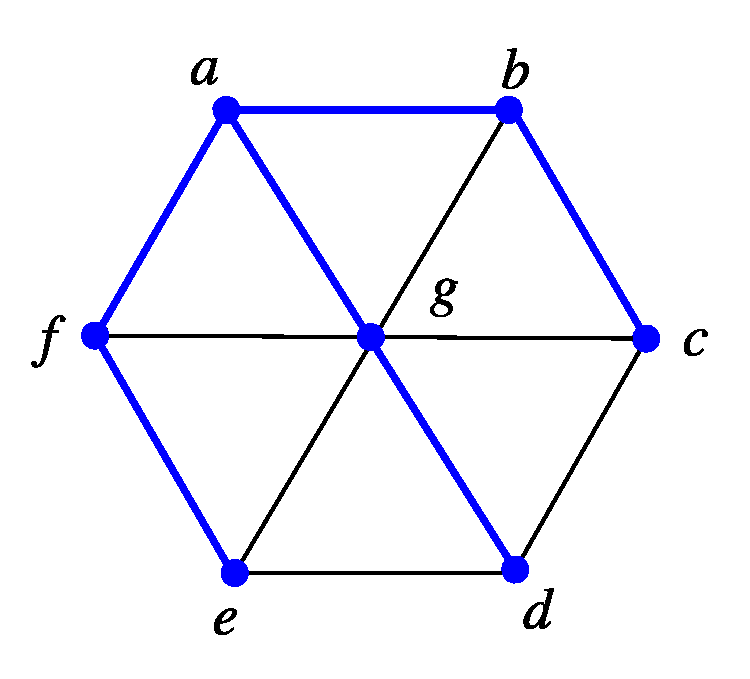
\includegraphics[scale = 0.6]{spanningtree.pdf}
\caption{Grafo $G$ con spanning tree (blu)}
\label{spanning}
\end{figure}

\begin{osservaz}
Se $G$ ammette spanning treee, allora $G$ è connesso. Infatti, se
$T$ è uno spanning tree per $G$, allora $V(T)\subseteq V(G)$ e
$E(T)\subseteq E(G)$. Quindi un cammino in $T$ è anche un cammino
in $G$. Poiché $T$ è connesso (per definizione di albero), allora
lo è anche $G$.
\end{osservaz}

\begin{tcolorbox}[title={Esistenza dell'albero di copertura per grafi connessi finiti}]
Se $G$ è un grafo finito connesso, allora esso ammette un albero di copertura.
$\\\\$
\textit{\textbf{Dimostrazione:}} Sia $G$ un grafo finito e connesso. Definiamo
l'insieme \[ \mathcal{C}:=\{C|C \text{ è un sottografo connesso di } G \text{ e } V(C)=V(G)\} \]
Mostriamo che in $\mathcal{C}$ esiste un albero.
Osserviamo che $\mathcal{C}\not=\varnothing$ perché $G\in\mathcal{C}$ grazie
all'ipotesi iniziale. Definiamo
\[ S:=\{n\in\mathbb{N} | n=|E(C)|, C\in\mathcal{C}\} \subset \mathbb{N} \]
Osserviamo che $|E(G)|\in S\Longrightarrow S\not=\varnothing$. Per il teorema del buon ordinamento dei naturali
\[ \exists m:=\min S \Longrightarrow \exists \overline{C}\in\mathcal{C}: |E(\overline{C})|=m\leq |E(C)| \quad \forall C\in\mathcal{C} \]
Mostriamo che $\overline{C}$ è un albero.
Supponiamo per assurdo che non lo sia. Quindi grazie al teorema 20.4 \[\exists e\in E(\overline{C}):
\overline{C}-e=(V(\overline{C}), E(\overline{C})\setminus\{e\})\in\mathcal{C}\]
Ma allora $|E(\overline{C}-e)| = |E(\overline{C})|-1 \in S$ e
avremmo $|E(\overline{C})|\leq |E(\overline{C})|-1$, che è assurdo.

\cvd
\end{tcolorbox}